\documentclass{standalone}

\usepackage{tikz}

\def \D { (0,0), (3,0), (6,0), (9,0), (2,1), (5,1), (1,2), (10,2), (3,3), (6,3), (9,3), (8,4), (11,4), (4,5), (7,5), (0,6), (3,6), (2,7), (5,7), (8,7), (1,8), (10,8), (6,9), (9,9), (2,10), (5,10), (8,10), (11,10) }

\def \A { (0,0), (9,0), (2,1), (5,1), (10,2), (3,3), (6,3), (4,5), (7,5), (0,6),  (5,7), (8,7), (1,8), (10,8) }

\def \B { (3,0), (6,0), (2,1), (10,2), (9,3), (8,4), (4,5), (3,6), (2,7), (10,8), (6,9), (9,9) }

\begin{document}
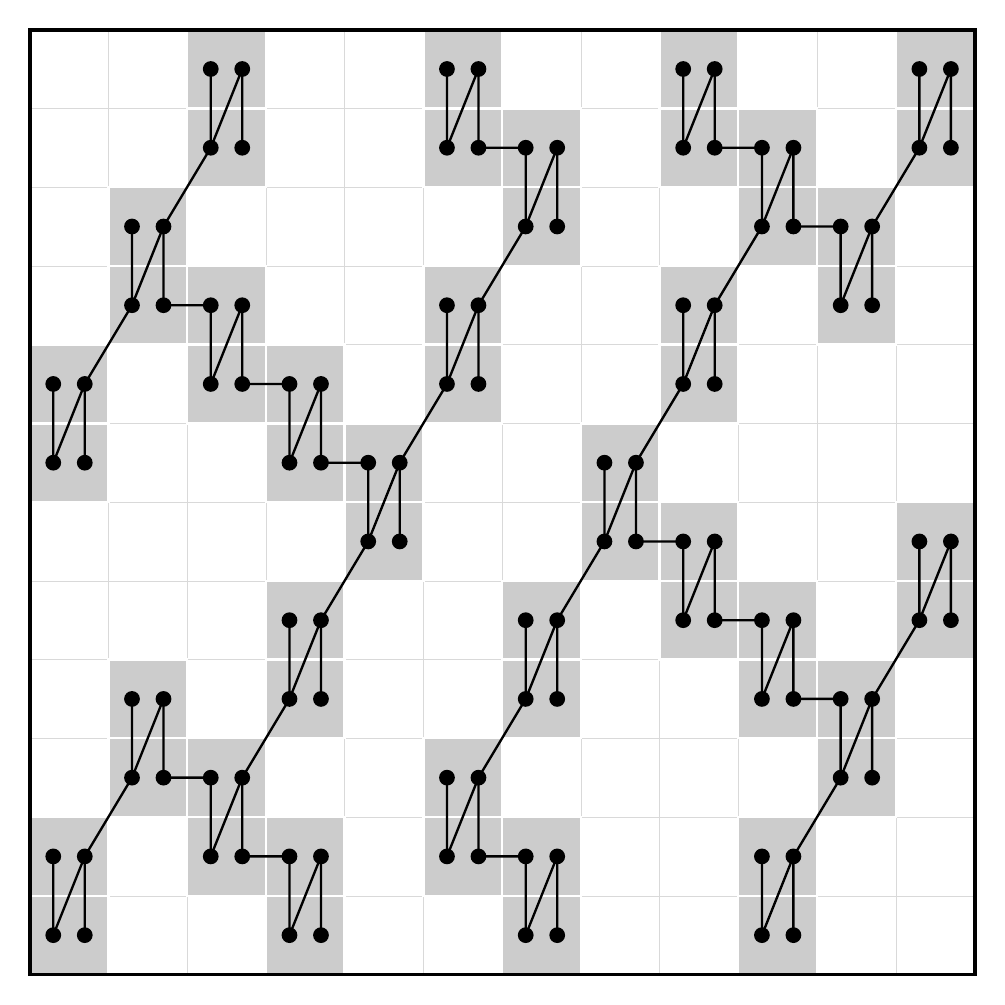
\begin{tikzpicture}
\draw[help lines, black!15] (0,0) grid (12,12);
\foreach \a in \D
    {\draw[black!0, fill=black!20, line width=0.3mm]
        \a rectangle +(1,1)
        \a++(0,1) rectangle +(1,1);
     \fill[black] foreach \b in 
        {(0.3, 0.5), (0.7, 0.5), (0.3, 1.5), (0.7, 1.5)}
        {\a++\b circle (1mm)};
     \draw[black, line width=0.3mm]
        \a++(0.3, 0.5)--+(0, 1)
        \a++(0.3, 0.5)--+(0.4, 1)
        \a++(0.7, 0.5)--+(0, 1);
    };
\draw[black, line width=0.3mm]
    foreach \a in \A
        {\a++(0.7, 1.5)--+(0.6, 1)}
    foreach \a in \B
        {\a++(0.3, 1.5)--+(-0.6, 0)};
\draw[black, line width=0.5mm] (0,0)rectangle (12,12);
\end{tikzpicture}
\end{document}